\documentclass[12pt]{standalone}
\usepackage[x11names, svgnames, rgb]{xcolor}
\usepackage[utf8]{inputenc}
\usepackage{tikz}
\usetikzlibrary{snakes,arrows,shapes}
\usepackage{amsmath}
%
%

%

%

\begin{document}
\pagestyle{empty}
%
%
%

\enlargethispage{100cm}
% Start of code
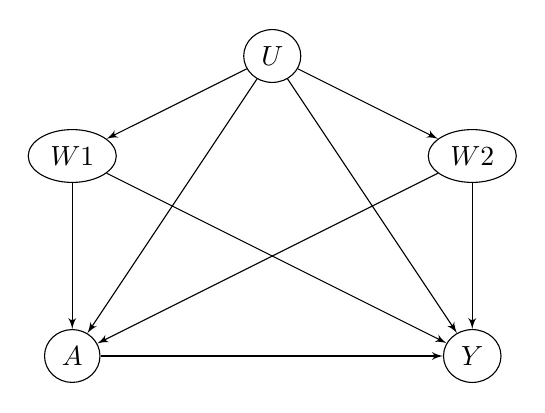
\begin{tikzpicture}[>=latex',line join=bevel,]
%%
\begin{scope}
  \pgfsetstrokecolor{black}
  \definecolor{strokecol}{rgb}{1.0,1.0,1.0};
  \pgfsetstrokecolor{strokecol}
  \definecolor{fillcol}{rgb}{1.0,1.0,1.0};
  \pgfsetfillcolor{fillcol}
  \filldraw (0.0bp,0.0bp) -- (0.0bp,128.0bp) -- (170.0bp,128.0bp) -- (170.0bp,0.0bp) -- cycle;
\end{scope}
\begin{scope}
  \pgfsetstrokecolor{black}
  \definecolor{strokecol}{rgb}{1.0,1.0,1.0};
  \pgfsetstrokecolor{strokecol}
  \definecolor{fillcol}{rgb}{1.0,1.0,1.0};
  \pgfsetfillcolor{fillcol}
  \filldraw (0.0bp,0.0bp) -- (0.0bp,128.0bp) -- (170.0bp,128.0bp) -- (170.0bp,0.0bp) -- cycle;
\end{scope}
\begin{scope}
  \pgfsetstrokecolor{black}
  \definecolor{strokecol}{rgb}{1.0,1.0,1.0};
  \pgfsetstrokecolor{strokecol}
  \definecolor{fillcol}{rgb}{1.0,1.0,1.0};
  \pgfsetfillcolor{fillcol}
  \filldraw (0.0bp,0.0bp) -- (0.0bp,128.0bp) -- (170.0bp,128.0bp) -- (170.0bp,0.0bp) -- cycle;
\end{scope}
  \node (A) at (13.0bp,10.0bp) [draw,ellipse] {$A$};
  \node (Y) at (157.0bp,10.0bp) [draw,ellipse] {$Y$};
  \node (U) at (85.0bp,118.0bp) [draw,ellipse] {$U$};
  \node (W2) at (157.0bp,82.0bp) [draw,ellipse] {$W2$};
  \node (W1) at (13.0bp,82.0bp) [draw,ellipse] {$W1$};
  \draw [->] (U) ..controls (65.407bp,108.2bp) and (47.878bp,99.439bp)  .. (W1);
  \draw [->] (W2) ..controls (120.11bp,63.555bp) and (61.204bp,34.102bp)  .. (A);
  \draw [->] (U) ..controls (102.48bp,91.781bp) and (130.05bp,50.428bp)  .. (Y);
  \draw [->] (U) ..controls (104.59bp,108.2bp) and (122.12bp,99.439bp)  .. (W2);
  \draw [->] (A) ..controls (47.019bp,10.0bp) and (105.41bp,10.0bp)  .. (Y);
  \draw [->] (U) ..controls (67.521bp,91.781bp) and (39.952bp,50.428bp)  .. (A);
  \draw [->] (W1) ..controls (13.0bp,58.102bp) and (13.0bp,42.852bp)  .. (A);
  \draw [->] (W2) ..controls (157.0bp,58.102bp) and (157.0bp,42.852bp)  .. (Y);
  \draw [->] (W1) ..controls (49.889bp,63.555bp) and (108.8bp,34.102bp)  .. (Y);
%
\end{tikzpicture}
% End of code

%
\end{document}
%



